\documentclass{article}

% Encodings, page setup, paragraph formatting, font
\usepackage[top=0.9in, bottom=1in, left=1.5in, right=1.5in]{geometry}
\usepackage[icelandic]{babel}
\usepackage[T1]{fontenc}
\usepackage[sc]{mathpazo}
\usepackage[parfill]{parskip}
\usepackage{cancel}
% Tables and lists
\usepackage{booktabs,tabularx}
\usepackage{multirow}
\usepackage{enumerate}
\usepackage{adjustbox}
\usepackage{multicol}
\usepackage{enumitem}
\usepackage{xcolor}
% Math
\usepackage{amsmath, amsfonts, amssymb, amsthm}
% Graphics
\usepackage{graphicx}
\usepackage{forest}
\usepackage{tikz}
\usetikzlibrary{positioning, shapes, arrows.meta}
% Custom Commands til að auðvelda lífið
\newcommand{\sv}{\textbf{Svar:}}
\newcommand{\bo}[1]{\textbf{#1}}
\newcommand{\enum}{\begin{enumerate}[label = \alph*.]}


\usepackage{listingsutf8}
\definecolor{commentcolor}{RGB}{255, 0, 255} % Bleikur
\definecolor{keywordcolor}{RGB}{139, 69, 19}   % Brúnn
\definecolor{stringcolor}{RGB}{0, 0, 255}      % Blár
\definecolor{numbercolor}{RGB}{0, 128, 0}      % Grænn
\definecolor{identifiercolor}{RGB}{0, 0, 255}
%Morpho
\lstdefinelanguage{CustomLang}{
    alsoletter={=},
    keywords={rec, fun, if, else, return},
    sensitive=true,
    comment=[l]{;;;},
    commentstyle=\color{commentcolor},
    morestring=[b]",
    stringstyle=\color{stringcolor},
}

\lstset{
    language=CustomLang,
    basicstyle=\ttfamily,
    keywordstyle=\color{keywordcolor},
    commentstyle=\color{commentcolor},
    identifierstyle=\color{identifiercolor},
    stringstyle=\color{stringcolor},   
    showstringspaces=false,
    numbers=none,
    tabsize=2,
    breaklines=true,
    columns=fullflexible,
    keepspaces=true,
    inputencoding=utf8, 
    extendedchars=true,  
    literate=
        {á}{{\'a}}1
        {ð}{{\dh}}1
        {é}{{\'e}}1
        {í}{{\'i}}1
        {ó}{{\'o}}1
        {ú}{{\'u}}1
        {ý}{{\'y}}1
        {þ}{{\th}}1
        {æ}{{\ae}}1
        {ö}{{\"o}}1
        {Á}{{\'A}}1
        {Ð}{{\DH}}1
        {É}{{\'E}}1
        {Í}{{\'I}}1
        {Ó}{{\'O}}1
        {Ú}{{\'U}}1
        {Ý}{{\'Y}}1
        {Þ}{{\TH}}1
        {Æ}{{\AE}}1
        {Ö}{{\"O}}1,
}


% Hyphenation
\hyphenpenalty=5000
% Page and section numbering
\setcounter{secnumdepth}{-1} 
\pagenumbering{gobble}
\title{Forritunarmál}
\author{Benjamín}
\date{11.27.2024}

\begin{document}

\maketitle
\begin{center}

\Huge{\textbf{TÖL304G Lokapróf}}


\LARGE{\textbf{Árið 2018}}


\vspace{5em}


\includegraphics[scale = 0.5]{myndir/bugun.jpg}
\end{center}


\newpage


\begin{center}
    \textbf{Hluti I - Bálkmótun o.fl.}

    \textbf{Svarið að minnsta kosti tveimur spurningum í þessum hluti - Munið að svara a.m.k. 10 spurningum í heild}
\end{center}

\section{1.}

Hverjar eftirfarandi fullyrðinga um lokanir eru sannar? Tvö röng svör gefa núll punkta.

\begin{itemize}
    \item[a)] Lokanir innihalda fallsbendi.
    \item[b)] Lokanir eru til í C.
    \item[c)] Lokanir eru til í Scheme.
    \item[d)] Lokanir eru til í CAML.
    \item[e)] Lokanir eru til í Morpho.
    \item[f)] Lokanir eru aðeins mögulegar ef vakningarfærslur eru í kös.
    \item[g)] Lokanir má nota til að utfæra strauma í Scheme.
    \item[h)] Lokanir innihalda tengihlekk(aðgangshlekk).
    \item[i)] Lokanir innihalda stýrihlekk.
    \item[j)] Lokanir innihalda straum.  
    \item[k)] Lokanir eru nauðsynlegar til að skila staðværu falli sem skilagildi falls í bálkmótuðum forritunarmálum.
    \item[l)] Lokanir eru nauðsynlegat til að senda staðvær föll sem viðföng í föll í bálkmótuðum forritunarmálum.        
\end{itemize}

\textbf{Svar}:



Förum í gegnum alla svarmöguleikana til að æfa okkur:

\enum
\item Lokanir innihalda fallsbendi?: Já Lokanir innihalda kóðann fyrir fallið (fallsbendil) og Umhverfið.
\item Lokanir eru til í C? Nei C styður ekki lokanir 
\item Lokanir eru til í Scheme? Já Scheme styður lokanir og notar þær mikið!
\item Lokanir eru til í CAML? Já CAML styður lokanir 
\item Lokanir eru til í Morpho? Já Morpho styður lokanir.
\item Lokanir eru einungis mögulegar ef vakningarfærslur eru í kös? Nei ekki satt.
\item Lokanir má nota til að utfæra strauma í Scheme? Já Straumar krefjast þess að við geymum útreikninga sem eru gerðir siðar, lokanir eru fullkomnar til þess.
\item Lokanir innihalda tengihlekk? Já, lokanir innihalda tengihlekk sem bendir á umhverfið þar sem fallið var skilgreint
\item Lokanir innihalda stýrihlekk? Neibb, Lokanir innihalda ekki stýrihlekk, þar sem stýrihlekkur tengist kallaröðinni, ekki umhverfinu.
\item Lokanir innihalda straum? Nei, lokanir sjálfar innihalda ekki straum.
\item Lokanir eru nauðsynlegar til að skila staðværu falli sem skilagildi falls í bálkmótuðum forritunarmálum? Já, til að skila staðværu falli og tryggja að það
      hafi aðganga að upprunalegu umhverfi sínu, þarf lokun.
\item Lokanir eru nauðsynlegar til að senda staðvær föll sem viðföng í föll í bálkmótuðum forritunarmálum?
      Sama röksemd og í k. til að fallið hafi aðgang að umhverfi sínu þegar það er notað sem viðfang, þarf lokun.

\end{enumerate}


\begin{tabularx}{\textwidth}{ |X|X|X|X|X|X|X|X|X|X|X|X|}
   \hline
   \textbf{a} & \textbf{b} & \textbf{c}  & \textbf{d} & \textbf{e}  & \textbf{f}  & \textbf{g}  & \textbf{h}  & \textbf{i}  & \textbf{j}  & \textbf{k}  & \textbf{l}  \\ \hline
    \bo{x} &  & \bo{x} & \bo{x} & \bo{x} &  & \bo{x} & \bo{x} &  &  & \bo{x} & \bo{x} \\ \hline
    
\end{tabularx}




\newpage

\section{2.}

Vakningarfærsla falls í bálkmótuðu forritunarmáli eins og Scheme inniheldur sum eftirfarandi atriða.
Hver? Eitt rangt svar gefur \underline{núll} stig.

\begin{enumerate}[label = \alph*)]
    \item Staðværar breytur fallsins.
    \item Staðværar breytur fallsins sem kallaði á fallið.
    \item Víðværar breytur sem eru aðgengilegar í fallinu.
    \item Skráarkerfi tölvunnar.
    \item Viðföng fallsins.
    \item Aðgangshlekk (tengihlekk).
    \item Stýrihlekk.
    \item Vendivistfang.
    \item Benda á öll föll sem hægt er að kalla á úr fallinu.
    \item Benda á allar lifandi vakningarfærslur.
    \item Alla hluti sem eru í kerfinu.
    \item Vakningarfærslur allra falla sem hægt er að kalla á.
    \item Nöfn allra falla sem hægt er að kalla á.
\end{enumerate}

\textbf{Svar}:

\begin{tabularx}{\textwidth}{ |X|X|X|X|X|X|X|X|X|X|X|X|X|}
    \hline
    \textbf{a} & \textbf{b} & \textbf{c}  & \textbf{d} & \textbf{e}  & \textbf{f}  & \textbf{g}  & \textbf{h}  & \textbf{i}  & \textbf{j}  & \textbf{k}  & \textbf{l} & \bo{m}  \\ \hline
     \bo{x} &  &  &  & \bo{x} & \bo{x}  & \bo{x} & \bo{x} &  &  &  &  &  \\ \hline
     
 \end{tabularx}

 \newpage

 \section{3.}
    Vakningarfærsla falls í bálkmótuðu forritunarmáli eins og Scheme inniheldur sum eftirfarandi atriða. Hver? Eitt rangt svar gefur \underline{núll} sitg.

    \begin{enumerate}[label = \alph*)]
        \item Staðværar breytur fallsins.
        \item Staðværar breytur fallsins sem kallaði á fallið
        \item Víðvlrar breytur sem eru aðgengilegar i fallinu.
        \item Skraarkerfi tölvunnar.
        \item viðföng fallsins.
        \item Aðgangshlekk (tengihlekk).
        \item Stýrihlekk.
        \item Vendivistfang.
        \item Benda á öll föll sem hægt er að kalla á úr fallinu.
        \item Benda á allar lifandi vakningarfærslur. 
        \item Alla hlutina sem til eru í kerfinu.
        \item Vakningarfærslur allra falla sem hægt er að kalla á.
        \item Nöfn allra falla sem hægt er að kalla á.
    \end{enumerate}

    \textbf{Svar}:

    \begin{tabularx}{\textwidth}{ |X|X|X|X|X|X|X|X|X|X|X|X|X|}
        \hline
        \textbf{a}  & \textbf{b}  & \textbf{c}  & \textbf{d}  & \textbf{e}  & \textbf{f}  & \textbf{g}  & \textbf{h}  & \textbf{i}  & \textbf{j}  & \textbf{k}  & \textbf{l} & \textbf{m}   \\ \hline
         & & & & & & & & & & & & \\ \hline
     \end{tabularx}

     \newpage

     \section{4.}
     Íhugið myndina sem sýnir földun falla P, Q, R, S og T.

     \begin{center}
        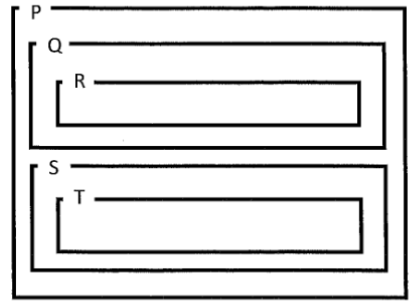
\includegraphics[scale = 1]{myndir/foldun.png}
     \end{center}

     Samsvarandi Scheme forritstexti er einnig sýndur í tveimur jafngildum útgáfum 
     hlið við hlið. 

     \begin{verbatim}
    (define ( P...)                        (define(P ...)
     (define (Q ...)                        (define(S ...)
      (define (R ...)                        (define (T...)
       ...[stifn R/body of R]                  ...[stofn T/body of T]
      )                                      )
      ...[stofn Q/body of Q]                 ...[stofn S/body of S]
     )                                      )
     (define (S ...)                        (define (Q ...)
      (define (T...)                         (define (R ...)
       ...[stofn T/body of T]                 ...[stofn R/body of R]
      )                                      )
      ...[stofn S/body of S]                 ...[stofn Q/body of Q]
     )                                      )
     ...[stofn P/body of P]                 ...[stofn P/body of P]
    )                                       )
     \end{verbatim}
    
     Fyllið út eftirfarandi töflur með því að setja krossa við sannar fullyrðingar.
     Eitt rangt svar gefur \underline{núll} í einkunn fyrir dæmið.

     \textbf{Svar}:

     Í þessu dæmi gildir að Það má alltaf kalla á ytra fall og beint barn. ekki barnabarn
     það skiptir ekki máli með kallanir hvort það

     kalla má á P úr:


     \begin{tabularx}{\textwidth}{ |X|X|X|X|X|}
        \hline
        \textbf{P}  & \textbf{Q}  & \textbf{R}  & \textbf{S}  & \textbf{T} \\ \hline
        \bo{x} & \bo{x} & \bo{x} & \bo{x} & \bo{x} \\ \hline
     \end{tabularx}


     kalla má á Q úr:

     
     \begin{tabularx}{\textwidth}{ |X|X|X|X|X|}
        \hline
        \textbf{P}  & \textbf{Q}  & \textbf{R}  & \textbf{S}  & \textbf{T} \\ \hline
        \bo{x} & \bo{x} & \bo{x} & \bo{x} & \bo{x} \\ \hline
     \end{tabularx}


     kalla má á R úr:

     
     \begin{tabularx}{\textwidth}{ |X|X|X|X|X|}
        \hline
        \textbf{P}  & \textbf{Q}  & \textbf{R}  & \textbf{S}  & \textbf{T} \\ \hline
         & \bo{x} & \bo{x} & \bo{x} & \bo{x} \\ \hline
     \end{tabularx}

     kalla má á S úr:

     
     \begin{tabularx}{\textwidth}{ |X|X|X|X|X|}
        \hline
        \textbf{P}  & \textbf{Q}  & \textbf{R}  & \textbf{S}  & \textbf{T} \\ \hline
         & \bo{x} & \bo{x} & \bo{x} & \bo{x} \\ \hline
     \end{tabularx}

     kalla má á T úr:

     
     \begin{tabularx}{\textwidth}{ |X|X|X|X|X|}
        \hline
        \textbf{P}  & \textbf{Q}  & \textbf{R}  & \textbf{S}  & \textbf{T} \\ \hline
         & \bo{x} & \bo{x}  & \bo{x}  & \bo{x}  \\ \hline
     \end{tabularx}

     Staðværar breytur í P má nota í:

     
     \begin{tabularx}{\textwidth}{ |X|X|X|X|X|}
        \hline
        \textbf{P}  & \textbf{Q}  & \textbf{R}  & \textbf{S}  & \textbf{T} \\ \hline
        \bo{x} & \bo{x} & \bo{x} & \bo{x} & \bo{x} \\ \hline
     \end{tabularx}


     Staðværar breytur í Q má nota í:

     
     \begin{tabularx}{\textwidth}{ |X|X|X|X|X|}
        \hline
        \textbf{P}  & \textbf{Q}  & \textbf{R}  & \textbf{S}  & \textbf{T} \\ \hline
         & \bo{x} & \bo{x} & & \\ \hline
     \end{tabularx}


     Staðværar breytur í R má nota í:

     
     \begin{tabularx}{\textwidth}{ |X|X|X|X|X|}
        \hline
        \textbf{P}  & \textbf{Q}  & \textbf{R}  & \textbf{S}  & \textbf{T} \\ \hline
         & & \bo{x} & & \\ \hline
     \end{tabularx}



     Staðværar breytur í S má nota í:

     
     \begin{tabularx}{\textwidth}{ |X|X|X|X|X|}
        \hline
        \textbf{P}  & \textbf{Q}  & \textbf{R}  & \textbf{S}  & \textbf{T} \\ \hline
         & & & \bo{x} & \bo{x} \\ \hline
     \end{tabularx}


     \newpage

     \section{5.}
     Eftirfarandi forritstexti er í einhverju ímynduðu forritunarmáli.
     \begin{verbatim}
        void f(x,y)
        {
            y = 3;
            print x,y;
            x = 2;
        }
        int i,a[10];
        for(int i= 0; i != 10; i++) a[i] = i +1;
        f(a[a[0]],a[0]);
        print a[0], a[1], a[2], a[3];
     \end{verbatim}

     Hvað skrifar þetta forrit (sex gildi í hvert skipti) ef viðföngin eru:

     \subsection{a)} Gildisviðföng 

    \sv 
    Viðföngin eru metin og gildin þeirra eru afrituð inn í fallið. Breytingar á viðföngum innan fallsins hafa engin áhrif á upprunalegu breyturnar.

    Svo þá munu gildin í f ekki breyta upprunulegu gildunum svo:
    \begin{verbatim}
        for lykkjan gerir
        a[0] = 1
        a[1] = 2
        a[2] = 3
        a[3] = 4
        a[4] = 5
        a[5] = 6
        a[6] = 7
        a[7] = 8
        a[8] = 9
        a[9] = 10
        svo 
        f(a[a[0]], a[0])
        gerir
        f(a[1], a[0])
        sem kallar á
        f(2, 1)

        svo prentað
        2 3
        1 2 3 4
    \end{verbatim}


     \subsection{b)} Tilvísunarviðföng
     Hér eru viðföngin send sem vísanir á upprunalegu breyturnar svo Breytingar
     á þeim innan fallsins hafa áhrif á upprunalegu breyturnar.

     svo þá er a[0] til a[9] upphafsstillt í 1 til 9

     en þegar f(a[a[0]], a[0]) er kallað þá breytir það stillingunni á a[0] og a[1]

     svo útprentað verður

     \begin{verbatim}
        2 3
        3 2 3 4
     \end{verbatim}


      


     \subsection{c)} Nafnviðföng


     Viðföngin eru send sem óútreiknaðar segðir og eru metin í hvert 

     svo inni i f:

     \begin{verbatim}
        1. y = 3
            a[0] = verður þá 3
        2. print x, y;
            x er a[a[0]], þar sem a[0] er núna 3, þannig að x er a[3] sem er 4
            y er a[0] sem er 3
            svo prentað er 4 3
        3. x = 2
           a[a[0]] =2;
           þar sem a[0] er 3 þá er þetta a[3] = 2 svo a[3] er 2
     \end{verbatim}

     Eftir fallið f þá prentum við 
     
     a[0], a[1], a[2], a[3];
     
     prentar :

     3 2 3 2


     Saman: 
     \bo{ 4 3 3 2 3 2}
     \newpage

     \begin{center}
        \textbf{Hluti II - Listavinnsla o.fl.}


        \textbf{Svarið að minnsta kosti tveimur spurningum i þessum hluta - Munið að svara a.m.k. 10 spurningum í heild}
     \end{center}

     \section{6.}
     Skrifið fall í Scheme, Caml, Morpho eða Haskell sem tekur eitt viðfang sem er listi lista af fleytitölum milli 0 og 1 og skilar tölu sem 
     er stærsta lággildi innri listanna, þ.e. stærst af þeim tölum sem fást 
     þegar fundinn er minnsta tala í hverjum innri lista. Þið skuluð reikna
     með því að hágildi í tóma menginu sé 0 og lággildi í tóma menginu sé 1.
     Munið fallslýsingar, eins og alltaf. Fallið þarf að skila viðeigandi 
     gildi bæði fyrir toman lista og fyrir lista sem einungis inniheldur tóma lista.

     \textbf{Svar:}

     \bo{í Scheme}:
     Ég ætla nota bara grunnskipanir

    \begin{lstlisting}
    ;;; Notkun: (min-i-lista lst)
    ;;; Fyrir: lst er listi af fleytitölum á milli 0 og 1
    ;;; Eftir: skilar minnsta gildi í listanum, eða 1 ef listinn er tómur
    (define (min-i-lista lst)
        (if (null? lst)
            1
            (min-helper (car lst) (cdr lst))
        )
    )

    ;;; Notkun: (min-helper current-min lst)
    ;;; Fyrir: current min er fleytitala, lst er listi af fleytitölum
    ;;; Eftir: Skilar minnsta gildi í listanum
    (define (min-helper current-min lst)
        (if (null? lst)
            current-min
            (let ((next-value (car lst)))
                (if (< next-value current-min)
                    (min-helper next-value (cdr lst))
                    (min-helper current-min (cdr lst))
                )
            )
        )
    )

    ;;; Notkun: (max-i-lista lst)
    ;;; Fyrir: lst er listi af fleytitölum 
    ;;; Gildi: Skilar stærsta gildinu í listanum, eða 0 ef listinn er tómur
    (define (max-i-lista lst)
        (if (null? lst)
            0
            (max-helper (car lst) (cdr lst))
        )
    )

    ;;; Notkun: (max-helper current-max lst)
    ;;; Fyrir: lst er listi af fleytitölum current-max er fleytitala
    ;;; Gildi: Skilar stærsta gildinu í listanum lst
    (define (max-helper current-max lst)
        (if (null? lst)
            current-max
            (let ((next-value (car lst)))
                (if (> next-value current-max)
                    (max-helper next-value (cdr lst))
                    (max-helper current-max (cdr lst))
                )
            )
        )
    )

    ;;; Notkun: (list-of-mins lst-of-lsts)
    ;;; Fyrir: lst-of-lsts er listi af fleytitölu listum fleytitölurnar eru á milli 0 og 1
    ;;; Eftir: skilar lista af minnstu gildum í öllum listunum
    (define (list-of-mins lst-of-lsts)
        (if (null? lst-of-lsts)
            '()
            (let((min-value (min-i-lista (car lst-of-lsts))))
                (cons min-value (list-of-mins (cdr lst-of-lsts)))
            )
        )
    )

    ;;; Notkun: (largest-min lst-of-lsts)
    ;;; Fyrir: lst-of-lsts er listi af listum af fleytitölum á milli 0 og 1
    ;;; Eftir: skilar stærsta lággildi innri listanna
    (define (largest-min lst-of-lsts)
        (let((mins (list-of-mins lst-of-lsts)))
            (max-i-lista mins)
        )
    )
    \end{lstlisting}



     \newpage 

     \section{7.}

     Skrifið fall Zip2 i Sheme, CAML, Morpho eða Haskell sem tekur 
     tvíundaraðgerð (fall) og tvo jafnlanga lista sem viðföng og skilar lista þeirra útkomna sem fást þegar tvíundaraðgerðinni er beitt á
     gildin í listunum, par fyrir par. Til dæmis, í Scheme þá ætti segðin
     (zip2 + '(1 2 3) '(4 5 6)) að skila listanum (5 7 9). Notið einungis
     einfaldar aðgerðir svo sem car, cdr, cons, null?

     \textbf{Svar}:

     \bo{Skrifum í scheme:}

     \begin{lstlisting}
     ;;; Notkun: (zip2 bin lst1 lst2)
     ;;; Fyrir: bin er tvíundaraðgerð, lst1 og lst2 eru jafnlangir listar.
     ;;; Eftir: skilar niðurstöðu tvíundaraðgerðinni á lst1 og lst2 í lista
     (define (zip2 bin lst1 lst2)
        (if (or (null? lst1) (null? lst2))
         '()
          (cons (bin (car lst1) (car lst2))
                (zip2 bin (cdr lst1) (cdr lst2))
          )
        )
     )
     \end{lstlisting}


     \newpage
     \section{8.}
     Skrifið ykkar eigin útgáfur af föllunum tveimur sem í CAML Light 
     eru kölluð \text{list\_it} og \text{list\_it}. Í Haskell eru þau kölluð foldl og foldr. 
     Þið megið skrifa þessi föll í Scheme, CAML, Morpho eða Haskell. Notið
     ekki lykkjur í Morpho. Kallið föllin myLeft og myRight. þið megið nota aðra röð viðfanga en í \text{it\_list og it\_list}. Sjáið til þess að a.m.k.
     annað fallið sé Halaendurkvæmt og tiltakið hvort það er. Notið 
     aðeins einföld innbygð föll svo sem car, cdr og null?.


     \textbf{Halaendurkvæma fallið er}:


     \textbf{Forritstexti (með lýsingum)}:

     \begin{lstlisting}
     ;;; Notkun: (myLeft bin init lst)
     ;;; Fyrir: 
     ;;;        - bin er tvíundaraðgerð
     ;;;        - init er upphafsgildi
     ;;;        - lst er listi af gildum
     ;;; Eftir: skilar niðurstöðu þess að fella lst frá vinstri með f og init
     (define (myLeft bin init lst)
        (if (null? lst)
        init
        (myLeft bin (bin (car lst)) (cdr lst))
        )
     )
     ;;; Notkun: (myRight bin init lst)
     ;;; Fyrir: 
     ;;;        - bin er tvíundaraðgerð
     ;;;        - init er upphafsgildi
     ;;;        - lst er listi af gildum
     ;;; Eftir: Skilar niðurstöðu þessa að fella lst frá hægri með f og init
     (define (myRight bin init lst)
        (if (null? lst)
            init
            (bin (car lst) (myRight bin init (cdr lst)))
        )   
     )
     \end{lstlisting}


     \newpage
     \section{9.}
     Skrifið halaendurkvæmt fall í Scheme, CAML, MORPHO eða Haskell
     sem tekur sem viðföng einn lista talna, x, auk tveggja talna $a$ og $b$,
     og skilar lista þeirra talna $z$ innan $x$ þar sem $a \leq z \leq$. þið munuð 
     vilja nota hjálparfall.


     \sv 


    \begin{lstlisting}
    ;;; Notkun: (filter-range x a b)
    ;;; Fyrir: 
    ;;;        - x er listi af tölum
    ;;;        - a og b eru tölur  
    ;;; Eftur: Skilar lista af þeim tölum z í x þar sem a <= z <= b.
    (define (filter-range x a b)
        (filter-range-helper x a b '())
    )

    ;;; Notkun: (filter-range-helper lst a b acc)
    ;;; Fyrir:
    ;;;        - lst er listi af tölum
    ;;;        - a, b eru tölur 
    ;;;        - acc er listi
    ;;; Eftir: Skilar lista af tölum í lst sem eru >= a og <= b.
    (define (filter-range-helper lst a b acc)
        (if (null? lst)
            (reverse acc)
            (let ((z (car lst)))
                (if (and (>= z a) (<= z b))
                    (filter-range-helper (cdr lst) a b (cons z acc))
                    (filter-range-helper (cdr lst) a b acc)
                )
            )
        )
    )

    \end{lstlisting}

     \newpage

     \begin{center}
     \bo{Hluti III - Einingarforritun o.fl.}

     \bo{Svarið að minnsta kosti tveimur spurningum í þessum hluta - Munið að svara a.m.k. 10 spurningum í heild}
     \end{center}


     \section{10.}
     Útfærið, að hluta, einingu fyrir fjölnota forgangsbiðröð í Morpho.
     Sýnið eftirfarandi.
     \begin{itemize}
        \item[a.] Hönnunarskjal sem inniheldur lýsingar (notkun/fyrir/eftir) fyrir
                  öll influtt og útflutt atriði einingarinnar.
        \item[b.] Smíð einingarinnar, þar sem sleppa má útfærslu allra 
                  aðgerða nema þeirri sem bætir gildi í forgangsbiðröðina.
                  Athugið að sýna þarf fastayrðingu gagna.
                  
     \end{itemize}
     Unnt skal vera að nota einingaraðgerðir til að búa til afbrigði af 
     einingunni sem gefa forgangsbiðraðir fyrir hvaða gildi sem er sem
     hafa viðeigandi samanburðarfall. Þið ráðið hvort forgangsbiðr-ðin er
     Útfærð sem hlutur eða ekki.

     \sv





    \begin{lstlisting}
    {;;;
    Hönnun
    ======

    Útflutt atriði
    --------------

    Notkun: pq = makePQ();
    Fyrir:  Ekkert
    Eftir:  pq er ný tóm forgangsbiðröð

    Innflutt atriði 
    ---------------

    Notkun: b = x <<== y;
    Fyrir:  x og y eru gildi af þeirri gerð sem við notendum
            sem lykla í forgangsbiðröðum
    Eftir:  b er satt ef lykillinn x má vera á undan lyklinum y

    Notkun: b = pq.isEmpty() ;
    Fyrir:  pq er forgangsbiðröð
    Eftir:  b er satt þá og því aðeins að pq sé tóm

    Notkun: g = pq.get();
    Fyrir:  pq er forgangsbiðröð, ekki tóm
    Eftir:  g er gildi sem var fjarlægt ú pq.
            g hafði lykil sem mátti vera fyrir framan
            lykla allra annara gilda í pq.

    Notkun: pq.add(k,g);
    Fyrir:  pq er forgangsbiðröð,
            k er lykilgildi þ.e. gildi sem er löglegt
    Eftir:  Búið er að bæta gildinu g í forgangsbiðröðina
            undir lyklinum k.

    
    ;;;}
    
    "pq.mmod" = 
    {{
    makePQ = 
        obj()
        {
            var list = [];
            {;;;
                Fastayrðing gagna:
                 Forgangsbiðröð sem inniheldur lykla/gilda-pör
                 (k1,g1),...,(kN,gN), þar sem fremri lyklar í 
                 rununni mega vera fyrir framan aftari lykla,
                 er geymd með list == [[k1$g1],...,[kN$gN]]
            ;;;}
            msg isEmpty()
                {
                    ...
                };
            msg put(k,g)
                {
                    ...
                };
            msg get()
                {
                    val res = tail(head(list));
                    list = tail(list);
                    return res;
                };
        }

    }}
    ;
    \end{lstlisting}


    \newpage
    \section{11.}
    Hverjar af eftirfarandi fullyrðingum eru í samræmi við meginregluna um upplýsingahuld? 
    Það gætu verið núll, ein eða fleiri. TVö röng svör gefa \underline{núll} stig.

    \enum
    \item Fastayrðing gagna einingar skal vera fullkomlega aðgengileg smiðum einingarinnar.
    \item Notendur einingar geta breytt gastayrðingu gagna einingarinnar.
    \item Gefa skal notendum einingar fullkomnar upplýsingar um smíð einingarinnar.
    \item Fastayrðing gagna einingar skal vera fullkomlega aðgengileg notendum einingarinnar.
    \item Fastayrðing gagna einingar skal ekki vera aðgengileg smiðum einingarinnar.
    \item Fastayrðing gagna einingar skal ekki vera aðgengileg notendum einingarinnar.
    \item Smiðir einingar geta breytt fastayrðingu gagna einingarinnar.
\end{enumerate}


    \sv

    
\begin{tabularx}{\textwidth}{ |X|X|X|X|X|X|X|}
    \hline
    \textbf{a}  & \textbf{b}  & \textbf{c}  & \textbf{d}  & \textbf{e}  & \textbf{f}  & \textbf{g} \\ \hline
     & & & & & & \\ \hline
 \end{tabularx}


 \newpage

 \section{12.}

 íhugið klasa A og B sem er undirklasi A. Gerið ráð fyrir að klasi A innihaldi boð f með forskilyrði $F_A$ og eftirskilyrði $E_A$.
 \begin{verbatim}
    //Notkun: x.f(...);
    //Fyrir:  F_A
    //Eftir:  E_A
 \end{verbatim}

 Gerið ráð fyrir að í klasa B sér bopip f endurskilgreint með
 \begin{verbatim}
    //Notkun: x.f(...);
    //Fyrir:  F_A
    //Eftir:  E_A
 \end{verbatim}

 Hvaða vensl þurfa þa gilda milli $F_A, E_A, F_B \text{ og } E_B$? Svarið þarf að
 vera tæmandi, þ.e. tilgreina nauðsyndleg og nægjanleg vendl.

 \sv

 \newpage

 \begin{center}
    \bo{Hluti IV - Ýmislegt}


    \bo{Svarið að minnsta kosti einni spurningu í þessum hluta 
    Munið að svara a.m.k. 10 spurningum í heild}
 \end{center}

 \section{13.}
 Lýsið ruslasöfnunaraðferðinni sem gengur undir nafninu 
 tilvísunartalning. Koma þarf fastayrðing gagna og undir hvaða 
 kringumstæðum minni er skilað.


 \sv

 \newpage
 \section{14.}
 Sýnið BNF, EBNF, samhengisfrjálsa mállýsingu (CFG) eða málrit
 fyrir mál lölegra segða yfir stafróið \text{\{x,+,(,)\}} þar sem $x$ er
 breytunafn og $+$ er tvíundaraðgerð

 Dæmi um streng í málinu.
 \begin{verbatim}
    x
    x + x
    x + (x)
    (((x)))
    x + (x + x + (x + x) + x) + x + x
 \end{verbatim}
 
 Dæmi um streng ekki í málinu.

\begin{verbatim}
    \epsilon (tómi strengurinn)
    (
    )
    +x
    ((x)
 \end{verbatim}



\end{document}